\documentclass[12pt,letterpaper]{article}
\usepackage{graphicx,textcomp}
\usepackage{natbib}
\usepackage{setspace}
\usepackage{fullpage}
\usepackage{color}
\usepackage[reqno]{amsmath}
\usepackage{amsthm}
\usepackage{fancyvrb}
\usepackage{amssymb,enumerate}
\usepackage[all]{xy}
\usepackage{endnotes}
\usepackage{lscape}
\newtheorem{com}{Comment}
\usepackage{float}
\usepackage{hyperref}
\newtheorem{lem} {Lemma}
\newtheorem{prop}{Proposition}
\newtheorem{thm}{Theorem}
\newtheorem{defn}{Definition}
\newtheorem{cor}{Corollary}
\newtheorem{obs}{Observation}
\usepackage[compact]{titlesec}
\usepackage{dcolumn}
\usepackage{tikz}
\usetikzlibrary{arrows}
\usepackage{multirow}
\usepackage{xcolor}
\newcolumntype{.}{D{.}{.}{-1}}
\newcolumntype{d}[1]{D{.}{.}{#1}}
\definecolor{light-gray}{gray}{0.65}
\usepackage{url}
\usepackage{listings}
\usepackage{color}

\definecolor{codegreen}{rgb}{0,0.6,0}
\definecolor{codegray}{rgb}{0.5,0.5,0.5}
\definecolor{codepurple}{rgb}{0.58,0,0.82}
\definecolor{backcolour}{rgb}{0.95,0.95,0.92}

\lstdefinestyle{mystyle}{
	backgroundcolor=\color{backcolour},   
	commentstyle=\color{codegreen},
	keywordstyle=\color{magenta},
	numberstyle=\tiny\color{codegray},
	stringstyle=\color{codepurple},
	basicstyle=\footnotesize,
	breakatwhitespace=false,         
	breaklines=true,                 
	captionpos=b,                    
	keepspaces=true,                 
	numbers=left,                    
	numbersep=5pt,                  
	showspaces=false,                
	showstringspaces=false,
	showtabs=false,                  
	tabsize=2
}
\lstset{style=mystyle}
\newcommand{\Sref}[1]{Section~\ref{#1}}
\newtheorem{hyp}{Hypothesis}

\title{Problem Set 3}
\date{Due: November 12, 2021}
\author{Applied Stats/Quant Methods 1}


\begin{document}
	\maketitle
	\section*{Instructions}
	\begin{itemize}
		\item Please show your work! You may lose points by simply writing in the answer. If the problem requires you to execute commands in \texttt{R}, please include the code you used to get your answers. Please also include the \texttt{.R} file that contains your code. If you are not sure if work needs to be shown for a particular problem, please ask.
		\item Your homework should be submitted electronically on GitHub in \texttt{.pdf} form.
		\item This problem set is due before class on Friday November 12, 2021. No late assignments will be accepted.
		\item Total available points for this homework is 80.
	\end{itemize}
		\lstinputlisting[language=R, firstline=40, lastline=41]{PS03_GC.R}
	
	\vspace{.25cm}
	
	\noindent In this problem set, you will run several regressions and create an add variable plot (see the lecture slides) in \texttt{R} using the \texttt{incumbents\_subset.csv} dataset. Include all of your code.
	
	\vspace{.5cm}
	\section*{Question 1} %(20 points)}
\vspace{.25cm}
\noindent We are interested in knowing how the difference in campaign spending between incumbent and challenger affects the incumbent's vote share. 
\begin{enumerate}
	\item Run a regression where the outcome variable is \texttt{voteshare} and the explanatory variable is \texttt{difflog}.	\vspace{5cm}
	\begin{verbatim}
	# read in incumbents data subset from online .csv
	incumbents <- read.csv("https://raw.githubusercontent.com/ASDS-TCD/StatsI_Fall2021/main/datasets/incumbents_subset.csv")
	# run regression model with voteshare regressed on difflog
	regression_model_problem2 <- lm(voteshare ~ difflog, data=incumbents)
	# get summary of model with coefficient estimates 
	summary(regression_model_problem1)
	
	Call:
	lm(formula = voteshare ~ difflog, data = incumbents)
	
	Residuals:
	Min       1Q   Median       3Q      Max 
	-0.26832 -0.05345 -0.00377  0.04780  0.32749 
	
	Coefficients:
	Estimate Std. Error t value Pr(>|t|)    
	(Intercept) 0.579031   0.002251  257.19   <2e-16 ***
	difflog     0.041666   0.000968   43.04   <2e-16 ***
	---
	Signif. codes:  
	0 ‘***’ 0.001 ‘**’ 0.01 ‘*’ 0.05 ‘.’ 0.1 ‘ ’ 1
	
	Residual standard error: 0.07867 on 3191 degrees of freedom
	Multiple R-squared:  0.3673,	Adjusted R-squared:  0.3671 
	F-statistic:  1853 on 1 and 3191 DF,  p-value: < 2.2e-16
	
	\end{verbatim}
	\item Make a scatterplot of the two variables and add the regression line. 
	\begin{verbatim}
		begin{figure}[width=0.9\textwidth]
		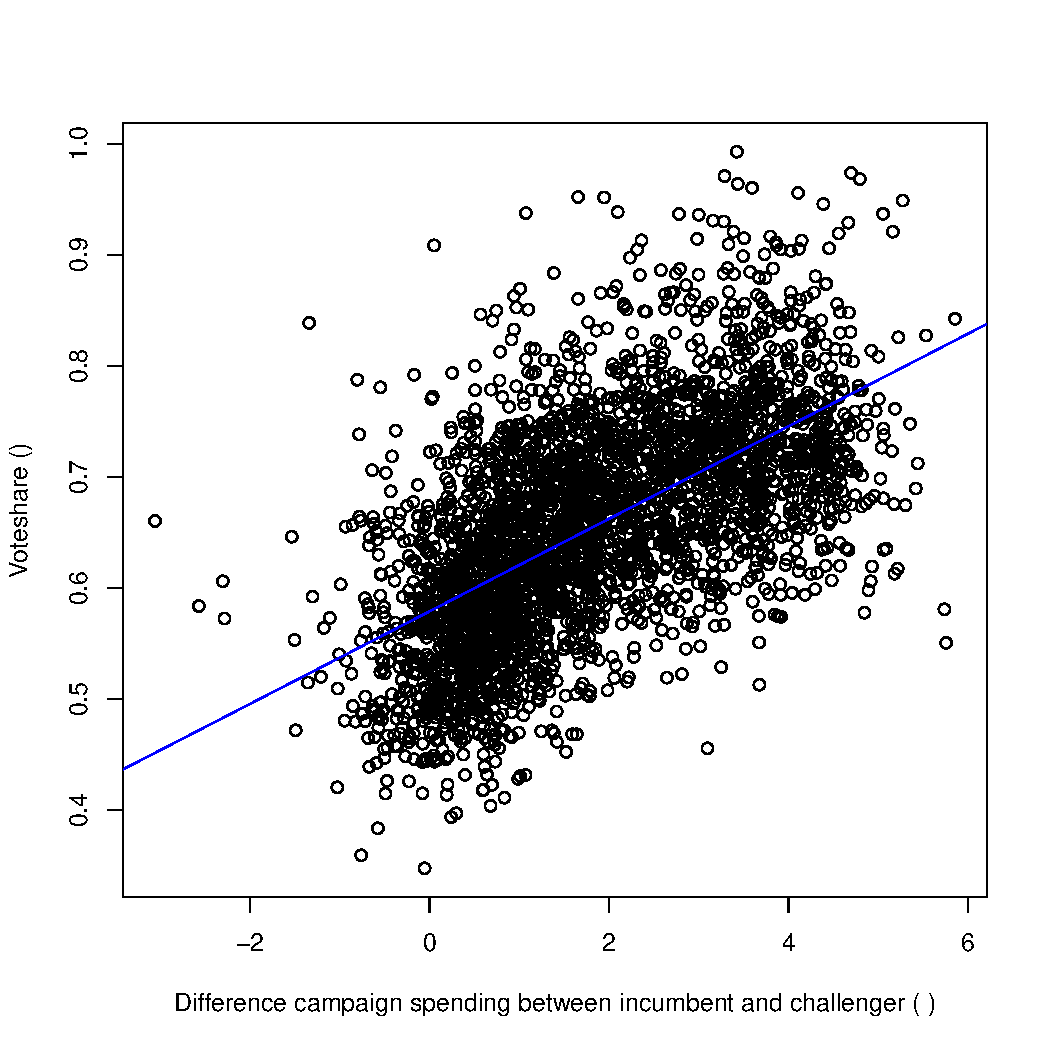
\includegraphics[width=8cm]{Figure1.pdf}
	\end{figure}
	plot(incumbents$difflog, incumbents$voteshare, 
	xlab = "Difference campaign spending between incumbent and challenger ( )", ylab = "Voteshare ()")
	
	abline(regression_model_problem1, col = "blue")
\end{verbatim}

\begin{figure}
	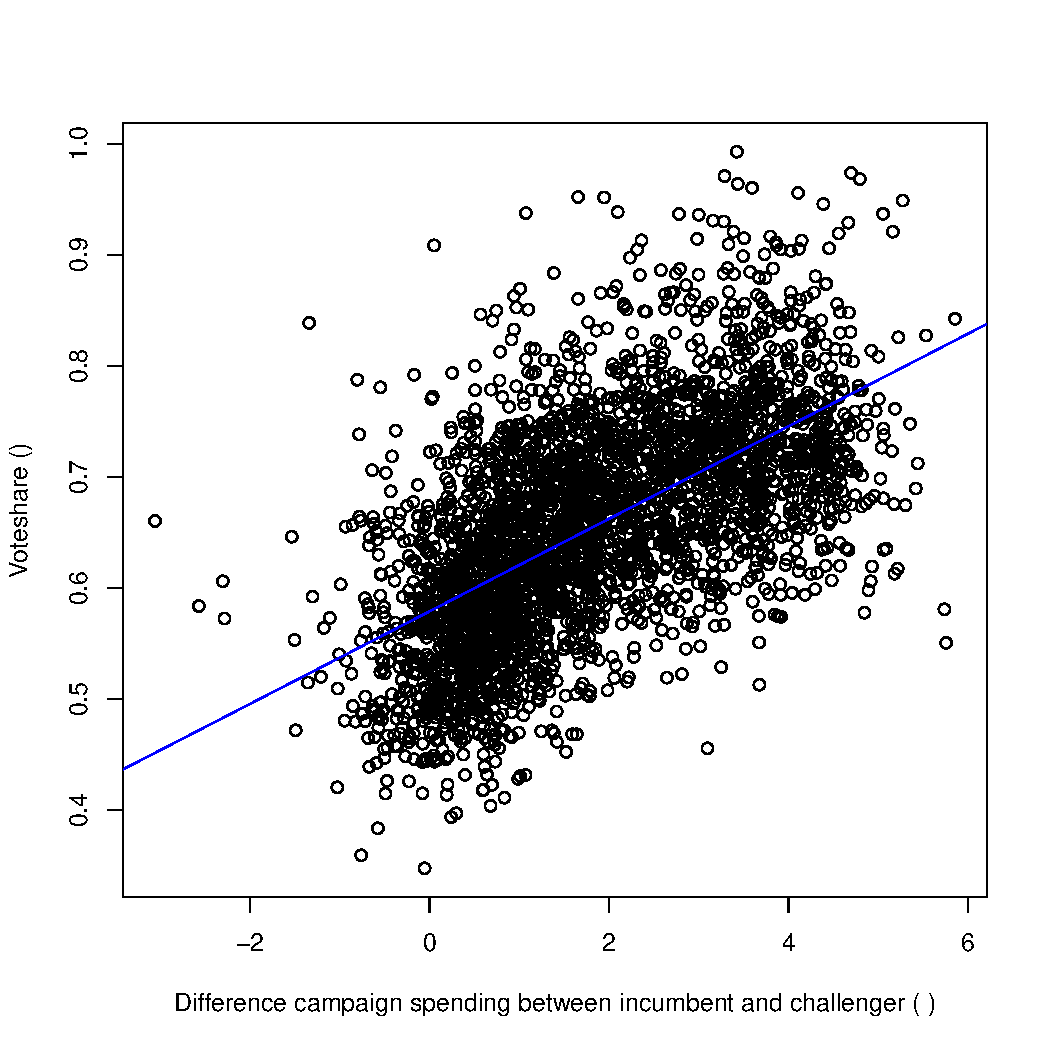
\includegraphics[width=0.9\textwidth]{Figure1.pdf}
\end{figure}
	\item Save the residuals of the model in a separate object.	
	
	\begin{verbatim}
		resids1 <- regression_model_problem1$residuals
\end{verbatim}
	\item Write the prediction equation.
	\begin{verbatim}
		#mean of outcome variable = the y-intercept or constant + slope of predictor1 multiplied by predictor 1 
		mean of outcome variable = t value of y intercept in table +  
\end{verbatim}
\end{enumerate}
\newpage


\section*{Question 2}% (20 points)}
\noindent We are interested in knowing how the difference between incumbent and challenger's spending and the vote share of the presidential candidate of the incumbent's party are related.	\vspace{.25cm}
\begin{enumerate}
\item Run a regression where the outcome variable is \texttt{presvote} and the explanatory variable is \texttt{difflog}.	
\begin{verbatim}
regression_model_problem2 <- lm(presvote ~ difflog, data=incumbents)

	summary(regression_model_problem2)
	
	Call:
	lm(formula = presvote ~ difflog, data = incumbents)
	
	Residuals:
	Min       1Q   Median       3Q      Max 
	-0.32196 -0.07407 -0.00102  0.07151  0.42743 
	
	Coefficients:
	Estimate Std. Error t value Pr(>|t|)    
	(Intercept) 0.507583   0.003161  160.60   <2e-16 ***
	difflog     0.023837   0.001359   17.54   <2e-16 ***
	---
	Signif. codes:  
	0 ‘***’ 0.001 ‘**’ 0.01 ‘*’ 0.05 ‘.’ 0.1 ‘ ’ 1
	
	Residual standard error: 0.1104 on 3191 degrees of freedom
	Multiple R-squared:  0.08795,	Adjusted R-squared:  0.08767 
	F-statistic: 307.7 on 1 and 3191 DF,  p-value: < 2.2e-16
	
	
\end{verbatim}
\item Make a scatterplot of the two variables and add the regression line. 	
\begin{verbatim}
	
	begin{figure}[width=0.9\textwidth]
	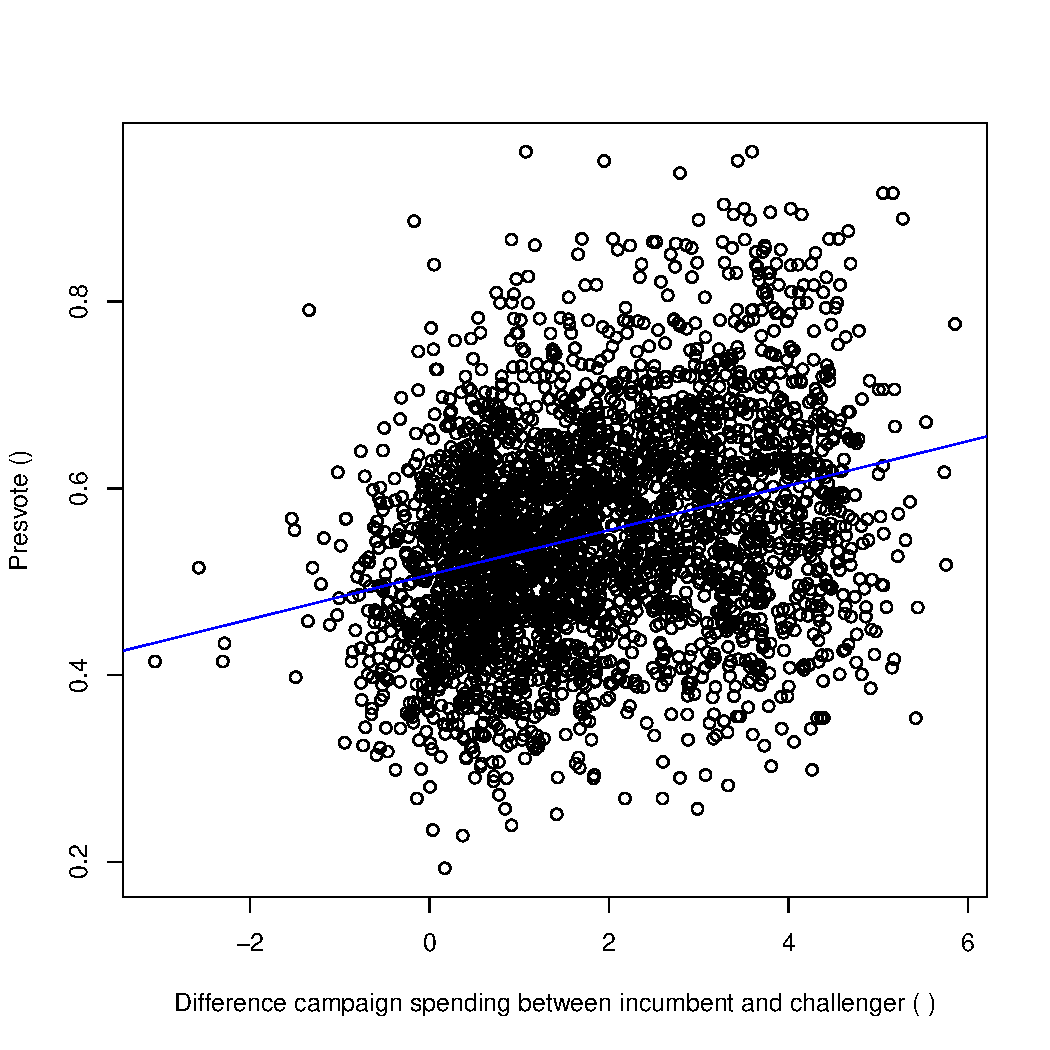
\includegraphics[width=8cm]{Figure2.pdf}
\end{figure}
	plot(incumbents$difflog, incumbents$presvote, 
	xlab = "Difference campaign spending between incumbent and challenger ( )", ylab = "Presvote ()")
	
	# Add the regression line to the scatterplot
	abline(regression_model_problem2, col = "blue")
	
	
\end{verbatim}

\begin{figure}
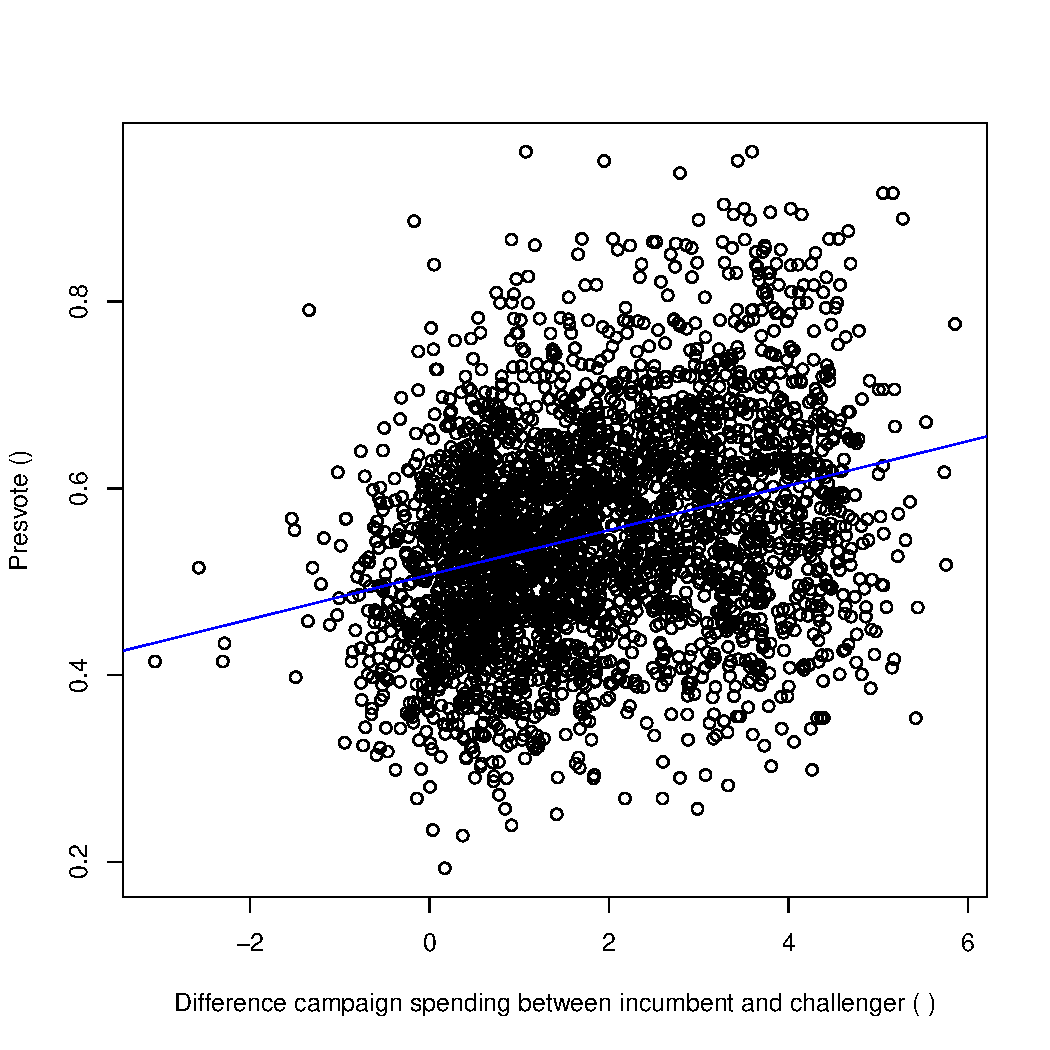
\includegraphics[width=9cm]{Figure2.pdf}
\end{figure}

\item Save the residuals of the model in a separate object.	
\begin{verbatim}
resids2 <- regression_model_problem2$residuals 
\end{verbatim}
\item Write the prediction equation.
\end{enumerate}
\begin{verbatim}
	#mean of outcome variable = the y-intercept or constant + slope of predictor1 multiplied by predictor 1 
	mean of outcome variable = 257.19 + 
\end{verbatim}

\newpage	
\section*{Question 3}% (20 points)}

\noindent We are interested in knowing how the vote share of the presidential candidate of the incumbent's party is associated with the incumbent's electoral success.
\vspace{.25cm}
\begin{enumerate}
\item Run a regression where the outcome variable is \texttt{voteshare} and the explanatory variable is \texttt{presvote}.

\begin{verbatim}
regression_model_problem3 <- lm(voteshare ~ presvote, data=incumbents)
	

# get summary of model with coefficient estimates 
summary(regression_model_problem3)
Call:
lm(formula = voteshare ~ presvote, data = incumbents)

Residuals:
Min       1Q   Median       3Q      Max 
-0.27330 -0.05888  0.00394  0.06148  0.41365 

Coefficients:
Estimate Std. Error t value Pr(>|t|)    
(Intercept) 0.441330   0.007599   58.08   <2e-16 ***
presvote    0.388018   0.013493   28.76   <2e-16 ***
---
Signif. codes:  
0 ‘***’ 0.001 ‘**’ 0.01 ‘*’ 0.05 ‘.’ 0.1 ‘ ’ 1

Residual standard error: 0.08815 on 3191 degrees of freedom
Multiple R-squared:  0.2058,	Adjusted R-squared:  0.2056 
F-statistic:   827 on 1 and 3191 DF,  p-value: < 2.2e-16

\end{verbatim}

\item Make a scatterplot of the two variables and add the regression line. 
\vspace{5cm}
\begin{verbatim}

	plot(incumbents$presvote, incumbents$voteshare, 
	xlab = "Difference campaign spending between incumbent and challenger ( )", ylab = "Voteshare ()")
	
	# Add the regression line to the scatterplot
	abline(regression_model_problem3, col = "blue")
	
\end{verbatim}
begin{figure}
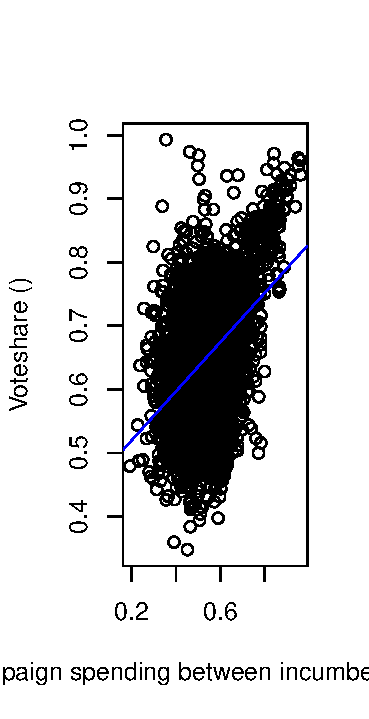
\includegraphics[width=8cm]
{Figure3.pdf}
\end{figure}


\item Write the prediction equation.
\end{enumerate}
	\begin{verbatim}
			#mean of outcome variable = the y-intercept or constant + slope of predictor1 multiplied by predictor 1 
		mean of outcome variable = 58.08 +
		
	\end{verbatim}


\newpage	
\section*{Question 4}% (20 points)}
\noindent The residuals from part (a) tell us how much of the variation in \texttt{voteshare} is $not$ explained by the difference in spending between incumbent and challenger. The residuals in part (b) tell us how much of the variation in \texttt{presvote} is $not$ explained by the difference in spending between incumbent and challenger in the district.
\begin{enumerate}
\item Run a regression where the outcome variable is the residuals from Question 1 and the explanatory variable is the residuals from Question 2.	
\begin{verbatim}
	regression_model_problem4 <- lm(resids1 ~ resids2 , data=incumbents)
	
	summary(regression_model_problem4)
	
	Call:
	lm(formula = resids1 ~ resids2, data = incumbents)
	
	Residuals:
	Min       1Q   Median       3Q      Max 
	-0.25928 -0.04737 -0.00121  0.04618  0.33126 
	
	Coefficients:
	Estimate Std. Error t value Pr(>|t|)    
	(Intercept) -4.860e-18  1.299e-03    0.00        1    
	resids2      2.569e-01  1.176e-02   21.84   <2e-16 ***
	---
	Signif. codes:  
	0 ‘***’ 0.001 ‘**’ 0.01 ‘*’ 0.05 ‘.’ 0.1 ‘ ’ 1
	
	Residual standard error: 0.07338 on 3191 degrees of freedom
	Multiple R-squared:   0.13,	Adjusted R-squared:  0.1298 
	F-statistic:   477 on 1 and 3191 DF,  p-value: < 2.2e-16
	
	
\end{verbatim}
\item Make a scatterplot of the two residuals and add the regression line. 	\vspace{6cm}
\begin{verbatim}

	
\end{verbatim}
	begin{figure}
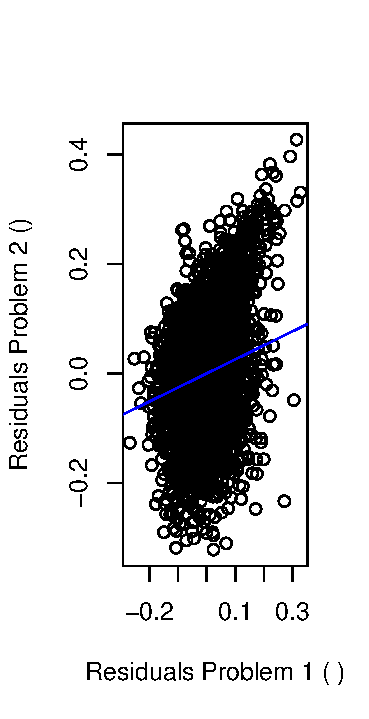
\includegraphics[width=8cm]{Figure4.pdf}
\end{figure}

\item Write the prediction equation.
\end{enumerate}
\begin{verbatim}
		#mean of outcome variable = the y-intercept or constant + slope of predictor1 multiplied by predictor 1 
	mean of outcome variable = 00.00 + 21.84 x 

\end{verbatim}
\newpage	

\section*{Question 5}% (20 points)}
\noindent What if the incumbent's vote share is affected by both the president's popularity and the difference in spending between incumbent and challenger? 
\begin{enumerate}
\item Run a regression where the outcome variable is the incumbent's \texttt{voteshare} and the explanatory variables are \texttt{difflog} and \texttt{presvote}.	
\begin{verbatim}
	regression_model_problem5 <- lm( voteshare ~ difflog + presvote, data=incumbents)
	\\
	View(regression_model_problem5)
	regression_model_problem5[["coefficients"]]
	(Intercept)     difflog    presvote 
	0.44864422  0.03554309  0.25687701 
	
	Reattempted
	Call:
	lm(formula = voteshare ~ difflog + presvote, data = incumbents)
	
	Residuals:
	Min       1Q   Median       3Q      Max 
	-0.25928 -0.04737 -0.00121  0.04618  0.33126 
	
	Coefficients:
	Estimate Std. Error t value Pr(>|t|)
	(Intercept) 0.4486442  0.0063297   70.88   <2e-16
	difflog     0.0355431  0.0009455   37.59   <2e-16
	presvote    0.2568770  0.0117637   21.84   <2e-16
	
	(Intercept) ***
	difflog     ***
	presvote    ***
	---
	Signif. codes:  
	0 ‘***’ 0.001 ‘**’ 0.01 ‘*’ 0.05 ‘.’ 0.1 ‘ ’ 1
	
	Residual standard error: 0.07339 on 3190 degrees of freedom
	Multiple R-squared:  0.4496,	Adjusted R-squared:  0.4493 
	F-statistic:  1303 on 2 and 3190 DF,  p-value: < 2.2e-16
	
\end{verbatim}
\item Write the prediction equation.	
\begin{verbatim}
#mean of outcome variable = the y-intercept or constant + slope of predictor1 multiplied by predictor1 + slope of predictor2 multiplied by predictor 2

mean of outcome variable = 0.4486442 + 0.03554309 x  + 0.256877 x 


\end{verbatim}
\item What is it in this output that is identical to the output in Question 4? Why do you think this is the case?%	\vspace{5cm}

 
%	\item Reflect on your finding. Don't write anything. Just think about it.
\end{enumerate}
\begin{verbatim}
	The mean of outcome variable - the slope numeric amount is the same in each equation due to the residuals object used.
\end{verbatim}



\end{document}